\documentclass[a4paper]{article}

\input ../header
\usepackage[np]{numprint}

\setlength{\multicolsep}{2pt}

\begin{document}

\title{Sujet A -- Internet}

\pagestyle{empty}

\date{}
\author{}

\maketitle{}
\thispagestyle{empty}

% Exercice définitions
\exo[1 point] Relier chaque mot à la bonne définition :

\begin{center}
  \begin{tabular}{@{}r@{\hspace{4cm}}l@{}}
    DNS $\bullet$ & $\bullet$ service qui permet de traduire\\
		  & \phantom{$\bullet$} un nom de domaine en adresse IP\\
		  &\\
    Cyclades $\bullet$ & $\bullet$ un des premiers navigateurs web\\
		       &\\
    Arpanet $\bullet$ & $\bullet$ projet expérimental français ayant pour\\
		      & \phantom{$\bullet$} but de créer un réseau d'ordinateurs\\
		      &\\
    Mosaic $\bullet$ & $\bullet$ premier réseau à transfert\\
		     & \phantom{$\bullet$} de paquets développé aux États-Unis\\
  \end{tabular}
\end{center}

\bigskip

\exo[1 point] Donner le nom d'un câble sous-marin arrivant en Polynésie.\rep{3}

\bigskip

% Petit exercice de conversion, rappels
\exo[2 points]\vspace*{-2mm}
\begin{enumerate}
  \item Qu'est-ce qu'un octet ?\rep{4}
  \item Convertir la quantité $30$ Mb (mégabits) en Mo (mégaoctets) puis en Go (gigaoctets).\rep{4}
\end{enumerate}

\bigskip

% Temps de téléchargement d'un fichier avec un forfait Fibre
\exo[4 points]\vspace*{-2mm}
Tearatamai profite de l'offre de connexion ci-dessous chez lui :

\begin{center}
  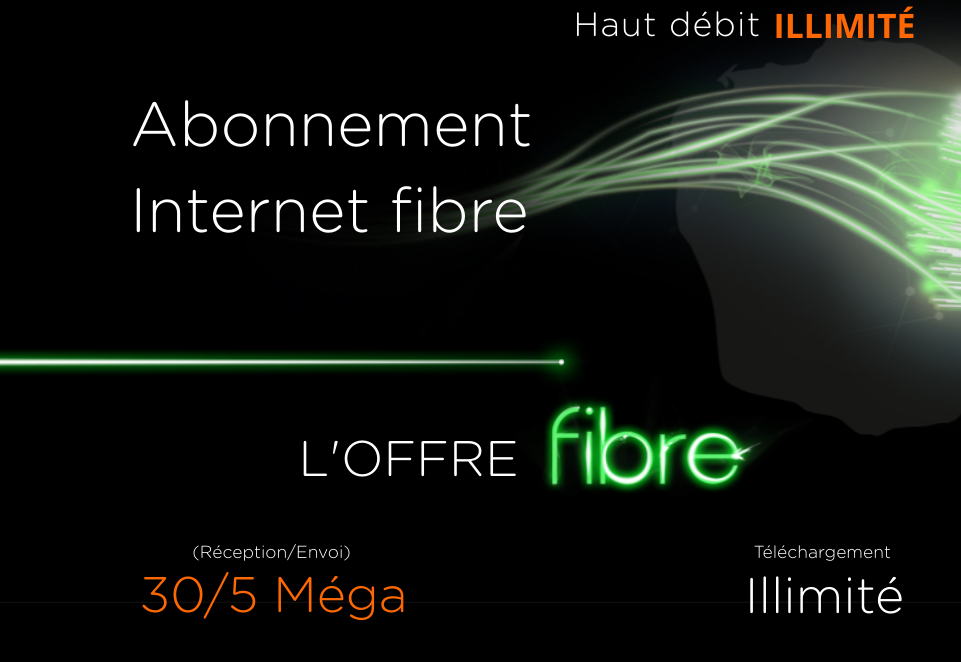
\includegraphics[width=12cm]{evaluation_2_seconde_15_sujet_A_viti_fibre.png}
\end{center}

Il peut donc télécharger à une vitesse de $30$ Mb par seconde.

\begin{enumerate}
  \item Louis demande à Tearatamai de lui télécharger une version de son film favori, \textit{Pokemon Detective Pikachu}. Combien de temps prendra le téléchargement, sachant que le fichier souhaité occupe $2,4$ Go ? (on supposera que Tearatamai le télécharge à la vitesse de $30$ Mb par seconde)\rep{10}
  \item Hirinaki souhaite ardemment aider Louis : elle aussi se met à télécharger le film. Sachant que Hirinaki peut télécharger à la vitesse de $6$ Mo par seconde, combien de temps mettra-t-elle ?\rep{10}
\end{enumerate}

\bigskip

% Comparaison avec ADSL
\exo[2 points]\vspace*{-2mm}
Lorsque Monsieur C. était plus jeune, il disposait d'une liaison par modem à $56$ kilobits par seconde. Combien de temps mettait-il pour télécharger un ficher MP3 de $8$ Mo ?\rep{10}

\end{document}
